\newpage
\section{绪论}

%——————————————————————图片格式——————————————————————	
\begin{figure}[htbp]
	\centering
	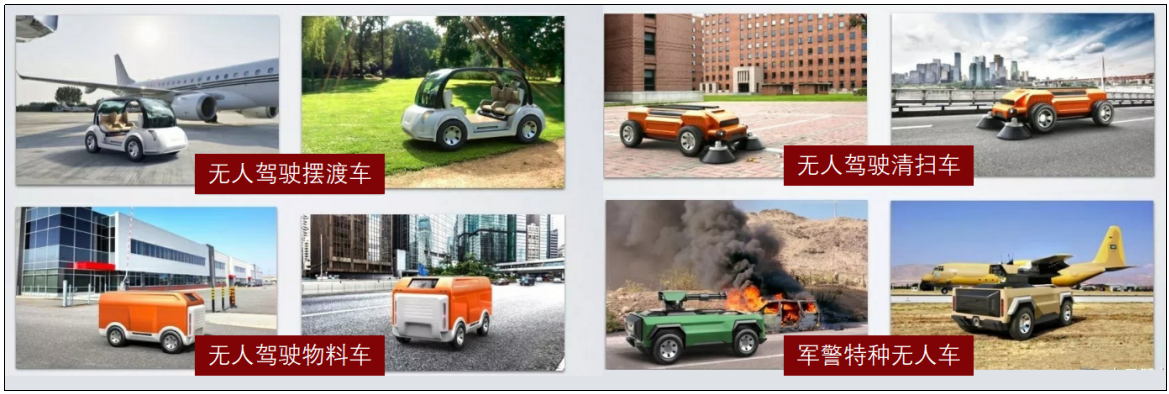
\includegraphics[width = 1\textwidth]{fig/wlknyy.png}
	\caption{未来可能应用}
	\label{wlknyy}
\end{figure}

%——————————————————————表格格式——————————————————————	
\begin{table}[htbp]
	\centering%表格居中
	\caption[centering]{The average daily use of sharing bicycles \protect\\and the number of bikes at the same period}%表格标题
	\label{共享单车日均使用总量与对应时间段的共享单车数量}%表格标签
	\begin{tabular}{ccc}
%	\begin{tabular}{C{4cm}C{4cm}C{3.5cm}}	
		\toprule
		\tabincell{c}{Averagedaily use\\(per 10000 people)} &\tabincell{c}{Sharing bicycles\\(per 10000 bikes)} &\tabincell{c}{Period}\\ 
		\midrule
		402.4 & 95 & 10.31$\sim$11.06 \\
		418.7 & 99 & 11.07$\sim$11.13 \\
		477.8 & 102 & 11.14$\sim$11.20 \\
		440.7 & 106 & 11.21$\sim$11.27 \\
		589.7 & 110 & 11.28$\sim$12.04 \\
		636.8 & 114 & 12.05$\sim$12.11 \\
		716.8 & 117 & 12.12$\sim$12.18 \\
		716.6 & 121 & 12.19$\sim$12.25 \\
		728.6 & 125 & 12.26$\sim$01.01 \\
		738.6 & 129 & 01.02$\sim$01.08 \\
		747.2 & 132 & 01.09$\sim$01.15 \\
		946.4 & 147 & 02.06$\sim$02.12 \\
		1047.1 & 151 & 02.13$\sim$02.19 \\
		1173.6 & 155 & 02.20$\sim$02.26 \\
		\bottomrule
	\end{tabular}
\end{table}

%——————————————————————对齐样式——————————————————————

一行对齐:\leftline{左对齐} \centerline{居中} \rightline{右对齐}
多行或者段落对齐:
左对齐 \begin{flushleft}...\end{flushleft}
居中 \begin{center}...\end{center}
右对齐 \begin{flushright}...\end{flushright}

%——————————————————————参考文献样式——————————————————————

%\section*{参考资料}
\addcontentsline{toc}{section}{参考文献}
\begin{thebibliography}{0}
		\bibitem{sj}
		赵瑜, 闫宏伟. 履带式行走机构设计分析和研究[J]. 新技术新工艺, 2010(5):50-53.
		
		\bibitem{dpsj}
		诸文农. 底盘设计[M]. 机械工业出版社, 2001.
	
\end{thebibliography}